\documentclass[draft.tex]{subfiles}
\begin{document}
\epigraph{“Why do you go away? So that you can come back. So that you can see the place you came from with new eyes and extra colors. And the people there see you differently, too. Coming back to where you started is not the same as never leaving.”}{Terry Pratchett}
Nonstandard Analysis and, more in general, nonstandard methods have always been considered a part of mathematical logic, mainly due to historical reasons. While nonstandard methods have, ever since the 60s, somehow detached themselves from the logical formalism Robinson had used, the \textit{unpleasant} logical flavour still permeates the theory, thus leading other mathematicians away. The consequences of this kind of stereotype (towards nonstandard methods and, more generally, towards mathematical logic) are uncountable, and while defeating the general suspicions mathematicians have towards logic might take more than a couple papers, something can (and ought to) be done for nonstandard methods. What follows is a characterization of nonstandard methods and, more in general, non-Archimedean mathematics that rests on topological methods and techniques instead of logical ones. $\Lambda-$limits will be introduced, and the natural setting for non-Archimedean mathematics --- a construction that parallels the construction of the reals as a completion of $\QQ$ --- will be built. All of the content of this chapter comes from \cite{NAM}.
%%%%%%%%%%%%%%%%%%%%%%%%%%%%%%%%%%%%%%%%%%%%%%%
\section{All in the $\Lambda-$afternoon: $\Lambda$-limits}
\begin{definition}
\label{def:lambdalim}
Let $(\fk{X}, \tau)$ be an Hausdorff topological space, and let $\cl{I}$ be a set, sometimes referred to as the \emph{parameter space}. Let $\cl{U}$ be a non-principal ultrafilter over $\cl{I}$, and $f: \cl{I} \to \fk{X}$ be a function. We say that $L \in \fk{X}$ is the \emph{$\Lambda$-limit of $f$}, and write
\begin{equation*}
    \lambdalim{f(\lambda)} = L,
\end{equation*}
if for every $V$ open neighbourhood of $L$ there exists a $Q \in \cl{U}$ such that $f[Q] \subseteq V.$
\end{definition}
This notion of $\Lambda-$limit is built as a natural generalization of a notion very common in general topology, that of convergence of a net.
\begin{remark}
A poset $(\cl{I}, \preceq)$ is called a \emph{directed set} if for any $A, B \in \cl{I}$ there exists a $C \in \cl{I}$ such that $A, B \preceq C.$ If $(\fk{X}, \tau)$ is a topological space, then a \emph{net over $\fk{X}$} is a function $f: \cl{I} \to \fk{X}$. Let $f: \cl{I} \to \fk{X}$ be a net over $(\fk{X}, \tau)$. Then \emph{$f$ converges to $L \in \fk{X}$}, in symbols $f \uparrow L$, if for every $V$ open neighbourhood of $L$, \emph{$f$ is eventually in $V$}, i.e. there exists a $\mu_0 \in \cl{I}$ such that for every $\mu \succeq \mu_0$, $f(\mu) \in V.$ $\Lambda-$limits, when taken with a fine\footnote{a ultrafilter on a directed set is fine if every set of the form $\{\mu: \mu_0 \preceq \mu\}$ belongs to the ultrafilter} ultrafilter $\cl{U}$, of nets generalize this notion (sometimes called \emph{Cauchy limit}). In fact, suppose $f: \cl{I} \to \fk{X}$ is a net over $\fk{X}$. If $f \uparrow L$, then for any $V$ open neighbourhood of $L$ there exists a $\mu_0 \in \cl{I}$ such that $f[\{\mu \in \cl{I}: \mu_0 \subseteq \mu\}] \subseteq V$. Since $\cl{U}$ is fine, $\{\mu \in \cl{I}: \mu_0 \subseteq \mu\} \in \cl{U}$, so $\lambdalim{f(\lambda)} = L.$
\end{remark}
\begin{remark}
$\Lambda-$limits could be defined topologically by giving $\cl{I} \cup \{\Lambda\}$, where $\Lambda \notin \cl{I},$ a topology that is discrete on $\cl{I}$ and that has as neighbourhoods of $\Lambda$ sets of the form $Q \cup \{\Lambda\}$ with $Q \in \cl{U}.$ In this case,
\begin{equation*}
    \lambdalim{f(\lambda)} = \lim\limits_{\lambda \to \Lambda} f(\lambda).
\end{equation*}
\end{remark}
%%%%%%%%%%%%%%%%%%%%%%%%%%%%%%%%%%%%%%%%%%%%%%%
\section{Down the $\Lambda$-hole: $\cl{I}$-completions}
We will now define a class of topological spaces that, due to the similarity with the '$\RR$ as a completion of $\QQ$' case, will be called $\cl{I}-$completions of the reals. These spaces will be, together with the intertwined notion of $\Lambda-$limit, the core of this theory and will provide an example of Non-Archimedean 'universe' where analysis (and other branches of mathematics) can be performed.
\begin{definition}
\label{def:completion}
Fix a non-principal ultrafilter $\cl{U}$ on $\cl{I}$. We will call a \emph{$\cl{I}$-completion of the reals} (and omit any reference to $\cl{U}$ whenever its specific properties are irrelevant) an Hausdorff topological space $(\RR_{\Lambda}, \tau)$ that satisfies the following conditions:
\begin{itemize}
    \item[$\Lambda$1.] $\cl{I} \times \RR$ is a dense subspace of $\completion$,
    \item[$\Lambda$2.] $\RR \subseteq \completion$ and for any $r \in \RR,$
    \begin{equation*}
        \lambdalim{(\lambda, r)} = r,
    \end{equation*}
    \item[$\Lambda$3.] for any function $f: \cl{I} \to \RR$ there exists the $\Lambda$-limit of $F(\lambda) = (\lambda, f(\lambda))$,
    \item[$\Lambda$4.] any two functions $f, g: \cl{I} \to \RR$ coincide on an element of $\cl{U}$ if and only if
    \begin{equation*}
        \lambdalim{F(\lambda)} =  \lambdalim{G(\lambda)}.
    \end{equation*}
\end{itemize}
\end{definition}
\begin{theorem}
\label{thm:existenceofcompl}
There exists a $\cl{I}$-completion of the reals.
\end{theorem}
\begin{proof}
We build a concrete example of $\cl{I}$-completion. Let $\cl{F}(\cl{I},\RR)$ be the algebra of functions over $\RR$. Let
\begin{equation*}
    I = \{f \in \cl{F}(\cl{I},\RR): \exists Q \in \cl{U} \ (\forall x \in Q \ (f(x) = 0))\}
\end{equation*}
be the ideal of functions that vanish on an element of the ultrafilter.
\begin{claim}
$I$ is a maximal ideal in $\cl{F}(\cl{I}, \RR)$.
\end{claim}
Let $J \supset I$ be another ideal, and let $g \in J \sm I$. Call $Z(g) = \{x \in \cl{I}: g(x) = 0\}$: since $g \notin I$, $Z(g) \notin \cl{U}$. Define
\begin{equation*}
    h(x) = \begin{cases}
    \frac{1}{g(x)} & \text{if} x \in \comp{Z(g)} \\
    0 & \text{if} x \in Z(g)
    \end{cases},
\end{equation*}
then since $J$ is an ideal $gh \in J$, and we have
\begin{equation*}
    (gh)(x) = \begin{cases}
    1 & \text{if} \ x \in \comp{Z(g)} \\
    0 & \text{if} \ x \in Z(g)
    \end{cases}.
\end{equation*}
$\cl{U}$ is an ultrafilter, so if $Z(g) \notin \cl{U}$ then $\comp{Z(g)} \in \cl{U}$, thus the following function
\begin{equation*}
    m(x) = \begin{cases}
    0 & \text{if} \ x \in \comp{Z(g)} \\
    1 & \text{if} \ x \in Z(g)
    \end{cases}
\end{equation*}
belongs to $I$, since it vanishes on $\comp{Z(g)} \in \cl{U}$. $J \supset I$, being an ideal, is closed under sum, so $(gh+m)(x) \in J$; the latter function is the identical function, so $J = \cl{F}(\cl{I},\RR)$, showing $I$ is maximal.
\par Call $\struct{K} = \cl{F}(\cl{I},\RR) / I$. As a consequence of the latter claim, it is a field (with the inherited operations). We are now ready to define $\completion$:
\begin{equation*}
    \completion = (\cl{I} \times \RR) \cup \struct{K}.
\end{equation*}
We give a basis for a topology on $\completion$:
\begin{equation*}
    \beta_{\Lambda} = \powerset{\cl{I} \times \RR} \cup \{\fk{B}^{Q}_{f}: Q \in \cl{U}, \ f \in \cl{F}(\cl{I}, \RR)\},
\end{equation*}
where for any $Q \in \cl{U}$ and $\varphi \in \cl{F}(\cl{I}, \RR)$,
\begin{equation*}
    \fk{B}^{Q}_{f} = \{(x, f(x)): x \in Q\} \cup \{[f]_{I}\}.
\end{equation*}
\begin{claim}
$\beta_{\Lambda}$ is the basis for an Hausdorff topology on $\completion$.
\end{claim}
We first show it is the basis for a topology: let $A, B \in \beta_{\Lambda}$ and $x \in A \cap B$. If $x \in \cl{I} \times \RR,$ then $(\cl{I} \times \RR) \cap A \cap B$ is a basis open set and $(\cl{I} \times \RR) \cap A \cap B \subseteq A \cap B$. On the other hand, if $x \in \struct{K}$ then $x = [f]_I$ for some function $f$ and $A = \fk{B}^{Q}_{g}$, $B = \fk{B}^{P}_{h}$ with $[h]_I = [g]_I = [f]_I$. Call $V \in \cl{U}$ the set on which these three functions coincide. Then $x \in \fk{B}^{V \cap Q \cap P}_{f} \subseteq A \cap B$.
\par To show that it is an Hausdorff topology, it is enough to show that $x \neq y \in \struct{K}$ can be separated by basis open sets. Let $x = [f]_I$ and $y = [g]_I$: since $x \neq y$, there exists a $Q \in \cl{U}$ such that $f(z) \neq g(z)$ for all $z \in \cl{U}$. It follows that $\fk{B}^{Q}_{f} \cap \fk{B}^{Q}_{g} = \emptyset$. 
\par We identify real numbers with the quotient class of constant functions.
\begin{claim}
For any function $f$ with real values,
\begin{equation*}
    \lambdalim{F(\lambda)} = [f]_I.
\end{equation*}
\end{claim}
Let $\fk{B}^{Q}_{g}$ be an open basis neighbourhood of $[f]_I$, so $[f]_I = [g]_I$. Call $P \in \cl{U}$ the set of parameters on which the two functions coincide. Then $F[Q \cap P] \subseteq \fk{B}^{Q}_{g}$.
\par With this claim in mind, we have that:
\begin{itemize}
    \item[$\Lambda$1.] $\cl{I} \times \RR$ is dense in $\completion$, since any basis open set overlaps with it,
    \item[$\Lambda$2.] follows from the identification of the real numbers with the equivalence classes of constant functions and the latter claim,
    \item[$\Lambda$3.] follows from the latter claim,
    \item[$\Lambda$4.] from the latter claim follows that if the limits coincide, $[f]_I = [g]_I$ and thus they coincide on an element of $\cl{U}$.
\end{itemize}
\end{proof}
\begin{figure}
\center

\tikzset{every picture/.style={line width=0.75pt}} %set default line width to 0.75pt        

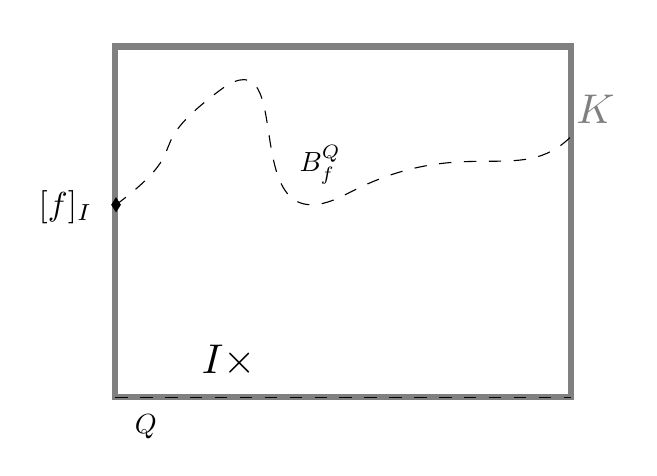
\begin{tikzpicture}[x=0.75pt,y=0.75pt,yscale=-1,xscale=1]
%uncomment if require: \path (0,361.3999938964844); %set diagram left start at 0, and has height of 361.3999938964844

%Shape: Rectangle [id:dp2943142001526706] 
\draw  [color={rgb, 255:red, 128; green, 128; blue, 128 }  ,draw opacity=1 ][line width=2.25]  (218,64.4) -- (437.5,64.4) -- (437.5,233.4) -- (218,233.4) -- cycle ;
%Curve Lines [id:da4597122169347565] 
\draw [color={rgb, 255:red, 0; green, 0; blue, 0 }  ,draw opacity=1 ] [dash pattern={on 4.5pt off 4.5pt}]  (218.34,140.62) .. controls (258.34,110.62) and (228.25,115.55) .. (268.25,85.55) .. controls (308.25,55.55) and (272.75,165.25) .. (329.5,135.4) .. controls (386.25,105.55) and (412.75,132.55) .. (437.75,107.55) ;


%Straight Lines [id:da5193460083502868] 
\draw [color={rgb, 255:red, 0; green, 0; blue, 0 }  ,draw opacity=1 ] [dash pattern={on 4.5pt off 4.5pt}]  (218,233.4) -- (437.5,233.4) ;


%Shape: Diamond [id:dp6794747639100498] 
\draw  [color={rgb, 255:red, 0; green, 0; blue, 0 }  ,draw opacity=1 ][fill={rgb, 255:red, 0; green, 0; blue, 0 }  ,fill opacity=1 ] (218.34,137.44) -- (220.37,140.62) -- (218.34,143.81) -- (216.32,140.62) -- cycle ;

% Text Node
\draw (272.67,215.73) node [scale=1.5]  {$\cl{I} \times \RR$};
% Text Node
\draw (449.33,94.67) node [scale=1.5,color={rgb, 255:red, 128; green, 128; blue, 128 }  ,opacity=1 ]  {$\struct{\textcolor[rgb]{0.5,0.5,0.5}{K}}$};
% Text Node
\draw (316.67,121.33) node [scale=1,color={rgb, 255:red, 0; green, 0; blue, 0 }  ,opacity=1 ]  {$\fk{B}^{Q}_{f}$};
% Text Node
\draw (232.67,247.5) node [scale=1,color={rgb, 255:red, 0; green, 0; blue, 0 }  ,opacity=1 ]  {$\textcolor[rgb]{0,0,0}{Q}$};
% Text Node
\draw (194,141.9) node [scale=1.2,color={rgb, 255:red, 0; green, 0; blue, 0 }  ,opacity=1 ]  {$\textcolor[rgb]{0,0,0}{[ f]_{I}}$};
\end{tikzpicture}
\caption{$\struct{K}$ can be thought of as ''points at infinity'' of $\cl{I}\times\RR$, and open sets of the form $\fk{B}^{Q}_{f}$ in $\completion$ as the union of the image of $Q \in \cl{U}$ under $(\lambda, f(\lambda))$ with the equivalence class $[f]_I$. Here $Q$ is a cofinite set that belongs to any non-principal ultrafilter.}
\end{figure}
%%%%%%%%%%%%%%%%%%%%%%%%%%%%%%%%%%%%%%%%%%%%%%%
\subsection{Ideals from a Caterpillar}
\label{subs:ideals}
The nature of a $\cl{I}$-completion of the reals strongly depends on the choice of the ultrafilter over $\cl{I}$. As we have seen in the proof of (\ref{thm:existenceofcompl}), an ultrafilter induces a maximal ideal in the algebra of real-valued functions $\cl{F}(\cl{I},\RR)$ (the ideal of functions that vanish on elements of the ultrafilter). The converse is true --- fixing a maximal ideal $M \subseteq \cl{F}(\cl{I},\RR)$ one can recover an ultrafilter on $\cl{I}$,
\begin{equation*}
    \cl{U}_{M} = \{f^{-1}(0): f \in M\}.
\end{equation*}
\begin{theorem}
Let $M \subseteq \cl{F}(\cl{I}, \RR)$ be a maximal ideal; then $\cl{U}_{M}$ is an ultrafilter.
\end{theorem}
\par This sort of duality implies that in order to define a notion of $\Lambda$-limit and $\cl{I}$-completion one can start from an ultrafilter or from a maximal ideal: this remark will be useful in Chapter 3, when we will build NAP spaces using ideals instead of filters.
%%%%%%%%%%%%%%%%%%%%%%%%%%%%%%%%%%%%%%%%%%%%%%%
\subsection{The Queen's Hyperreal-Field}
We now consider a fixed $\cl{I}-$completion of the reals, $\completion$. Inside any such space there is a special subspace that we will denote by $\struct{K} = \{ \lambdalim{(\lambda, f(\lambda))}: f \in \cl{F}(\cl{I},\RR)\}.$ We call this subspace the \emph{hyperreal field}, since it can be equipped with two complete operations:
\begin{equation}
\label{eq:field}
    \lambdalim{(\lambda, f(\lambda))} \ast \lambdalim{(\lambda, g(\lambda))} = \lambdalim{(\lambda, f(\lambda)\ast g(\lambda))},
\end{equation}
with $\ast \in \{+, \cdot\}$. $\struct{K}$ naturally contains $\RR$ as a subfield.
\begin{theorem}
The set $\struct{K}$ with the operations defined in (\ref{eq:field}) is a field.
\end{theorem}
\begin{proof}
The only interesting proof is that of the existence of multiplicative inverses. Namely, if $x \neq 0$ is an element of $\struct{K}$, then $x = \lambdalim{(\lambda, f(\lambda))}$ and since $\completion$ is Hausdorff there exists a (basis) open set separating $x$ and $0$ --- in particular, there exists a $Q \in \cl{U}$ such that for every $\lambda \in Q$, $f(\lambda) \neq 0$. This means we can define a function
\begin{equation*}
    g(\lambda) =
    \begin{cases}
    1, & \text{if} \ x \notin Q, \\
    \frac{1}{f(\lambda)}, & \text{if} \ x \in Q,
    \end{cases}
\end{equation*}
whose limit will be the inverse of $x$ (in fact, $\lambdalim{(\lambda, f(\lambda)\cdot g(\lambda))} = 1$).
\end{proof}
$\struct{K}$ can be ordered in the natural way, i.e. saying that
\begin{equation*}
    \lambdalim{(\lambda, f(\lambda))} \leq \lambdalim{(\lambda, g(\lambda))}
\end{equation*}
if and only if $\{\lambda \in \cl{I}: f(\lambda) \leq g(\lambda)\} \in \cl{U}$.
\par We now show that the idea of $\struct{K}$ as disjoint ''points at infinity'' is preserved in the general setting.
\begin{lemma}
Let $\completion$ be a $\cl{I}-$completion of the reals, then $\finset{\RR} \times \RR \cap \struct{K} = \emptyset$.
\end{lemma}
\begin{proof}
Suppose not, so there exists a function $f: \cl{I} \to \RR$ such that $\lambdalim{(\lambda, f(\lambda))} = (\overline{\lambda}, \overline{r}) \in \cl{I} \times \RR$. By definition of $\Lambda-$limit, there exists a $Q \in \cl{U}$ such that for every $\lambda \in Q$ $(\lambda, f(\lambda)) = (\overline{\lambda}, \overline{r})$. In particular, $Q = \{\overline{\lambda}\}$, which is absurd since $\cl{U}$ is non-principal.
\end{proof}
Call \emph{minimal} every $\cl{I}-$completion of the reals of the form $(\cl{I} \times \RR) \sqcup \struct{K}$.
\par As it is use in topology, we kept writing $\completion$ to denote a $\cl{I}-$completion of the reals but we shouldn't forget that the same set could be a $\cl{I}-$completion of the reals for different choices of topologies. There is, however, a choice that we wish to isolate:
\begin{definition}
Let $\completion$ be a $\cl{I}-$completion of the reals for a certain topology $\tau$. We will call \emph{slim topology} the topology $\tau_{\Lambda}$ generated by
\begin{equation*}
    \powerset{\cl{I} \times \RR} \cup \{\fk{B}^{Q}_{f}: Q \in \cl{U}, \ f \in \cl{F}(\cl{I},\RR)\},
\end{equation*}
where the open sets $\fk{B}^{Q}_{f}$ are defined precisely as in (\ref{thm:existenceofcompl}). Call $(\completion, \tau_{\Lambda})$ a \emph{canonical} $\cl{I}-$completion of the reals.
\end{definition}
Canonical $\cl{I}-$completions are well-behaved in the sense that just like $\overline{\cl{I}\times \RR} = \completion$, the closure of subsets of $\cl{I} \times \RR$ is made up by the subset and the limits of functions that are eventually in the subset:
\begin{theorem}
Let $\completion$ be a canonical $\cl{I}-$completion of the reals, then for every $B \subseteq \cl{I} \times \RR$, we have 
\begin{equation*}
\overline{B} = B \cup \{\lambdalim{(\lambda, f(\lambda))}: \exists Q \in \cl{U} \ (\forall z \in Q \ (z,f(z)) \in B)\}.
\end{equation*}
\end{theorem}
\begin{proof}
Let $f: \cl{I} \to \RR$ and $B \subseteq \cl{I} \times \RR:$ call $B(f) = \{\lambda \in \cl{I}: (\lambda, f(\lambda)) \in B\}.$ Call $\phi = \lambdalim{(\lambda, f(\lambda))}.$
\par If $B(f) \in \cl{U}$, then every open neighbourhood of $\phi$ meets, by definition, $B$, so $\phi \in \overline{B}$; on the other hand, if $B(f) \notin \cl{U}$ then $\fk{B}^{B(f)}_{f}$ is disjoint from $B$, thus $\phi \notin \overline{B}$.
\end{proof}
\par If we consider a minimal canonical $\cl{I}-$completion of the reals, it turns out this topological path is equivalent to a variant of a well-known construction we considered in the previous chapter.
\begin{definition}
Let $\RR_{\cl{U}}$ be the quotient set of $\RR^{\cl{I}}$ by the equivalence relationship $f \equiv g$ if and only if $\{\lambda \in \cl{I}: f(\lambda) = g(\lambda)\} \in \cl{U}$.
\end{definition}
\begin{theorem}
$\struct{K}$ and $\RR_{\cl{U}}$ are isomorphic as fields.
\end{theorem}
\begin{proof}
Let $\mathfrak{i}: \struct{K} \to \RR_{\cl{U}}$ be defined by $   \mathfrak{i}(\lambdalim{(\lambda, f(\lambda))} = [f]$. Then $\mathfrak{i}$ respects operations by their very definitions, it is injective due to $\Lambda4$ and surjective due to $\struct{K}$ being exactly the set of all $\Lambda-$limits.
\end{proof}
%%%%%%%%%%%%%%%%%%%%%%%%%%%%%%%%%%%%%%%%%%%%%%%
\section{Refrain: superstructures (II)}
Classical nonstandard methods can be extended to superstructures, in order to allow for a more general use of mathematical objects. The same happens for $\Lambda-$limits:
\begin{definition}
Let $\phi: \cl{I} \to V_{\omega}(\RR)$ be a \emph{bounded} function if there exists a maximal rank $n \in \NN$, i.e. a natural number such that for every $\lambda \in \cl{I}$, $\phi(\lambda) \in V_{n}(\RR)$. We define $\Lambda-$limits for bounded functions by induction. If $n = 0,$ these were already defined. Let $\phi$ be bounded of maximal rank $n,$ then
\begin{equation*}
    \lambdalim{(\lambda, \phi(\lambda))} = \big\{\lambdalim{(\lambda, f(\lambda))}: f: \cl{I} \to V_{n-1}(\RR) \ \mathrm{and} \ \forall \lambda \in \cl{I}, f(\lambda) \in \phi(\lambda)\big\} \in V_{\omega}(\struct{K}).
\end{equation*}
\end{definition}
$\Lambda-$limits of bounded functions are called \emph{internal}, while every other element is called \emph{external}. $\struct{K}$ is internal, while $\RR$ and $\struct{K} \sm \RR$ are external. This approach to superstructures ends up being strictly related to the general one exposed in the previous chapter:
\begin{theorem}
Let $\star: V_{\omega}(\RR) \to V_{\omega}(\struct{K})$ be defined by
\begin{equation*}
    \ns{x} = \lambdalim{(\lambda, x)}
\end{equation*}
where the $\Lambda-$limit is taken at the rank of $x$. Then $\langle V_{\omega}(\RR), V_{\omega}(\struct{K}), \star \rangle$ is a nonstandard universe.
\end{theorem}
\end{document}